\documentclass[]{article}
\usepackage{lmodern}
\usepackage{amssymb,amsmath}
\usepackage{ifxetex,ifluatex}
\usepackage{fixltx2e} % provides \textsubscript
\ifnum 0\ifxetex 1\fi\ifluatex 1\fi=0 % if pdftex
  \usepackage[T1]{fontenc}
  \usepackage[utf8]{inputenc}
\else % if luatex or xelatex
  \ifxetex
    \usepackage{mathspec}
  \else
    \usepackage{fontspec}
  \fi
  \defaultfontfeatures{Ligatures=TeX,Scale=MatchLowercase}
\fi
% use upquote if available, for straight quotes in verbatim environments
\IfFileExists{upquote.sty}{\usepackage{upquote}}{}
% use microtype if available
\IfFileExists{microtype.sty}{%
\usepackage[]{microtype}
\UseMicrotypeSet[protrusion]{basicmath} % disable protrusion for tt fonts
}{}
\PassOptionsToPackage{hyphens}{url} % url is loaded by hyperref
\usepackage[unicode=true]{hyperref}
\hypersetup{
            pdfborder={0 0 0},
            breaklinks=true}
\urlstyle{same}  % don't use monospace font for urls
\usepackage[margin=1in]{geometry}
\usepackage{longtable,booktabs}
% Fix footnotes in tables (requires footnote package)
\IfFileExists{footnote.sty}{\usepackage{footnote}\makesavenoteenv{long table}}{}
\usepackage{graphicx,grffile}
\makeatletter
\def\maxwidth{\ifdim\Gin@nat@width>\linewidth\linewidth\else\Gin@nat@width\fi}
\def\maxheight{\ifdim\Gin@nat@height>\textheight\textheight\else\Gin@nat@height\fi}
\makeatother
% Scale images if necessary, so that they will not overflow the page
% margins by default, and it is still possible to overwrite the defaults
% using explicit options in \includegraphics[width, height, ...]{}
\setkeys{Gin}{width=\maxwidth,height=\maxheight,keepaspectratio}
\IfFileExists{parskip.sty}{%
\usepackage{parskip}
}{% else
\setlength{\parindent}{0pt}
\setlength{\parskip}{6pt plus 2pt minus 1pt}
}
\setlength{\emergencystretch}{3em}  % prevent overfull lines
\providecommand{\tightlist}{%
  \setlength{\itemsep}{0pt}\setlength{\parskip}{0pt}}
\setcounter{secnumdepth}{5}
% Redefines (sub)paragraphs to behave more like sections
\ifx\paragraph\undefined\else
\let\oldparagraph\paragraph
\renewcommand{\paragraph}[1]{\oldparagraph{#1}\mbox{}}
\fi
\ifx\subparagraph\undefined\else
\let\oldsubparagraph\subparagraph
\renewcommand{\subparagraph}[1]{\oldsubparagraph{#1}\mbox{}}
\fi

% set default figure placement to htbp
\makeatletter
\def\fps@figure{htbp}
\makeatother

\usepackage{float}
\usepackage{titling}
\usepackage{caption} 
\usepackage{amsmath}
\usepackage{booktabs}
\captionsetup[table]{skip=8pt}
\usepackage{abstract}
  \renewcommand{\abstractnamefont}{\normalfont\large\bfseries}
\usepackage{booktabs}
\usepackage{longtable}
\usepackage{array}
\usepackage{multirow}
\usepackage{wrapfig}
\usepackage{float}
\usepackage{colortbl}
\usepackage{pdflscape}
\usepackage{tabu}
\usepackage{threeparttable}
\usepackage{threeparttablex}
\usepackage[normalem]{ulem}
\usepackage{makecell}
\usepackage{xcolor}

\author{}
\date{\vspace{-2.5em}}

\begin{document}

\begin{flushleft}
\LARGE{\textbf{Country Level Indicators of Suicide Risk:\\ Data Analysis \& Decision Support for Policy Makers}}\\
\vspace*{2\baselineskip}
\Large{Project Report: Georgia Tech ISyE 6414 - Dr. Yajun Mei}\\
\vspace*{3\baselineskip}
\Large{\textbf{Team Members}}\\
Samuel Garcia\\
Michael Szostak\\ 
Osman Ghandour\\ 
Peter Williams\\
\vspace*{2\baselineskip}
\Large{\textbf{Report Date}}\\
April 21, 2020
\newpage
\end{flushleft}

{
\setcounter{tocdepth}{2}
\tableofcontents
}
\newpage

\begin{abstract}
\bigskip
Relying on open source data from the World Health Organization and other non-governmental bodies, we highlight trends and related to country-level measures of suicide globally. A descriptive model is formulated that identifies a set of meaningful factors and measures that highlights some intuitive relationships between country-level suicide rates and other indicators such as income, alcohol consumption, and the presence of a country level suicide prevention strategy.   

An initial framework for data-driven decision support for policy makers is presented with recommendations including the identification and ongoing monitoring of meaningful factors and measures related to suicide prevention. The hope is that this can provide some introductory guidance for those managing health related planning activities and priorities related to this topic.   

An overview of the sources of data, and process of collection, of data related to suicide at the country level is also described briefly, along with a description of some  ancillary datasets that were employed to augment and enrich insights. The intention of these descriptions is to make further research and data analysis on this topic more accessible to other interested researchers and data analysts in the future.  

\end{abstract}

\section{Research Motivation}\label{research-motivation}

According to the \emph{World Health Organization}, (``Suicide: One
Person Dies Every 40 Seconds'' 2019) one person dies every 40 seconds
from suicide. It is the second leading cause of death among teenagers
and adults aged 15-29 years. Despite the staggering number of suicides
happening worldwide, just 38 governments worldwide have a national
suicide prevention strategy.

Each of these deaths are tragic, and sadly also preventable. For every
suicide, there are many more attempts, and previous suicide attempts are
the single most important predictor or risk factor for future suicide
attempts. (``Suicide: Key Facts'' 2019) The possibility of prevention
and the scale of the problem highlight the need for policy makers, at
the national level, to understand the factors that contribute to suicide
not only in their own nations but also globally.

\section{Variables \& Data Sources}\label{variables-data-sources}

The core dataset we plan to rely on comes directly from the \emph{World
Health Organization} and is referenced below. 


The key measure of
interest for our study is the \emph{the age-standardized suicide rate}
by country, which is defined as \emph{a weighted average of the
age-specific mortality rates per 100,000 persons, where the weights are
the proportions of persons in the corresponding age groups of the WHO
standard population.} (``Suicide Rate Estimates, Age-Standardized
Estimates by Country'' 2019) The data consists of country-level measures
of suicides rates. These estimates of
age-standardized suicide rates were taken in the year with the most recent available data for each country.
In addition to
relying on the core suicide rate statistics provided above, we
intend to append country-level data
from ancillary data sources. We consider the following
data:

\begin{enumerate}
\def\labelenumi{\arabic{enumi}.}
\item
  Current Health Expenditure as a percentage of GDP - 
  \emph{World Bank}

\item
  Labor force participation rate, female to male ratio - 
  \emph{World Bank}
  
\item
  GDP per capita, PPP - 
  \emph{OECD} 
\item
  Liters of Alcohol per capita - 
 \emph{United
  Nations Development Programme}
  
\item
  Prevelence of a Suicide Prevention Strategy - 
  \emph{World Health Organization}
  
  Psychiatrists in mental health, per 100,000 population - 
  \emph{World Health Organization}
  
\item
  Mental hospitals, per 100,000 population - 
  \emph{World Health Organization}
    
Note that detailed descriptions of the data and the source links can be found in the appendix. 


 
\end{enumerate}

\begin{center}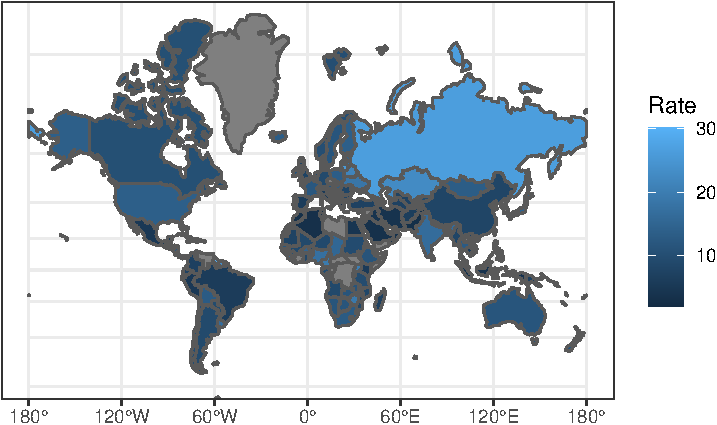
\includegraphics{Project_Report_files/figure-latex/world_map_plot-1} \end{center}

\begin{center}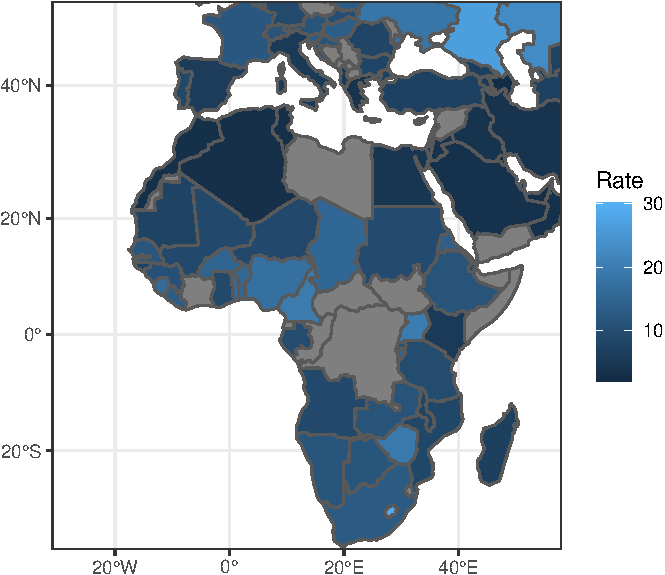
\includegraphics{Project_Report_files/figure-latex/africa_map_plot-1} \end{center}

\begin{center}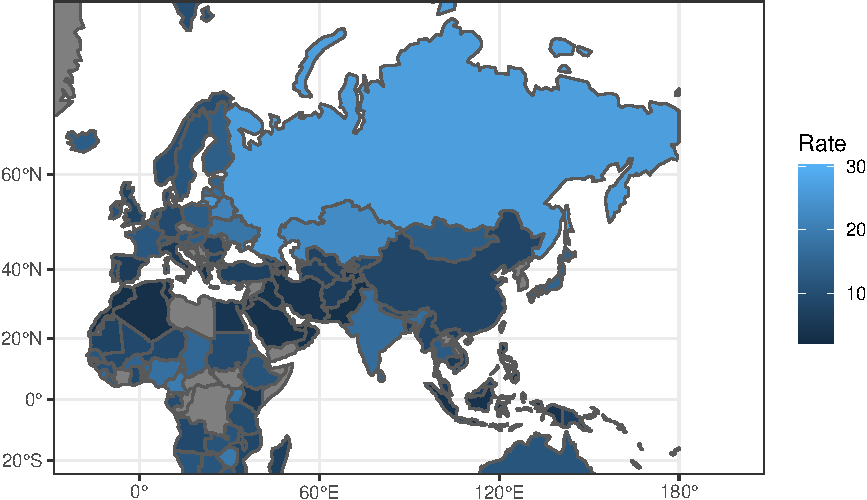
\includegraphics{Project_Report_files/figure-latex/russia_map_plot-1} \end{center}

\section{Modeling \& Assumptions}\label{modeling-assumptions}

\emph{explain (and justify) your proposed methods or models.}

\section{Quantifying Impact of Measures on
Suicide}\label{quantifying-impact-of-measures-on-suicide}

\emph{present key findings when executing the proposed methods or
models. For the benefit of readability, detailed results should be
placed in the Appendix. Reference of computer softwares to implement
your proposed methods or models (even it is a web page) should be
given.}

\subsection{Identifying, Describing and Monitoring Country Level
Indicators Is Critical~for
Effective~Decision-Making~Support}\label{identifying-describing-and-monitoring-country-level-indicators-is-criticalfor-effectivedecision-makingsupport}

\begin{table}[H]
\centering 
\caption{Decision Support Framework for Policy Makers}
\
\begin{tabular}{p{5cm}p{10cm}}  
\hline  
   Area of Focus  & Decision Support  \\   
\hline 
 Identifying \& Quantifying Measures and Indicators of Country Level Suicide Rates &  Using a model to describe the relationships between country-level indicators and suicide rates to help policy makers identify what variables are important and putting context around how to monitor them \\   
 \hline 
Incorporating Domain Knowledge and Expertise of Subject Matter Experts & Allows policy makers to correlate indicators with country-level suicide related outcomes in context of qualitative insights from experts in the field \\   
\hline 
Insight Gathering, Analysis and Support Policy Maker Decisions & Integrating data and insights and providing inital context to help policy makers to frame longer term health planning activities and policies \\
\hline 
\end{tabular} 
\end{table}

\subsubsection{Quantifying Impact: Income, GDP per
person}\label{quantifying-impact-income-gdp-per-person}

Insights

Our model indicates the presence of a significant relationship between a
measure of income (country-level GDP per person) and suicide~

Countries with lower per person income, tend to have higher incidence of
suicide when controlling for other variables in our model*

Based on our estimates, an approximate 10\% increase in income
corresponds to a 2\% decrease in suicide rate at the country level for
the typical country

\begin{center}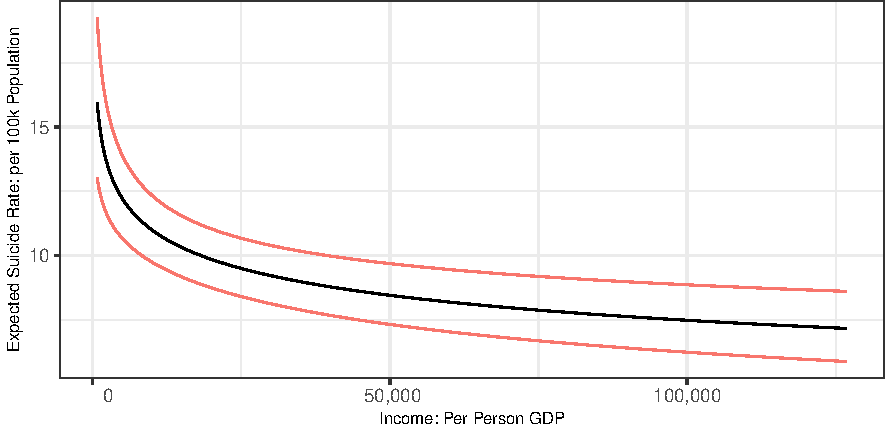
\includegraphics{Project_Report_files/figure-latex/agdp_plot-1} \end{center}

\subsubsection{Quantifying Impact: Alcohol
Consumption:}\label{quantifying-impact-alcohol-consumption}

Insights

Our model indicates the presence of a significant relationship between a
measure of alcohol consumption (liters per year)

Countries with higher levels of alcohol consumption income, tend to have
higher incidence of suicide when controlling for other variables in our
model*

Based on our estimates, an approximate 4\% increase in alcohol
consumption corresponds to a 2\% increase in suicide rate at the country
level for the typical country (\textgreater{}4 liters per year)

Alcohol consumption was the most impactful and significant indicator of
country-level suicide rate in our analysis

\begin{center}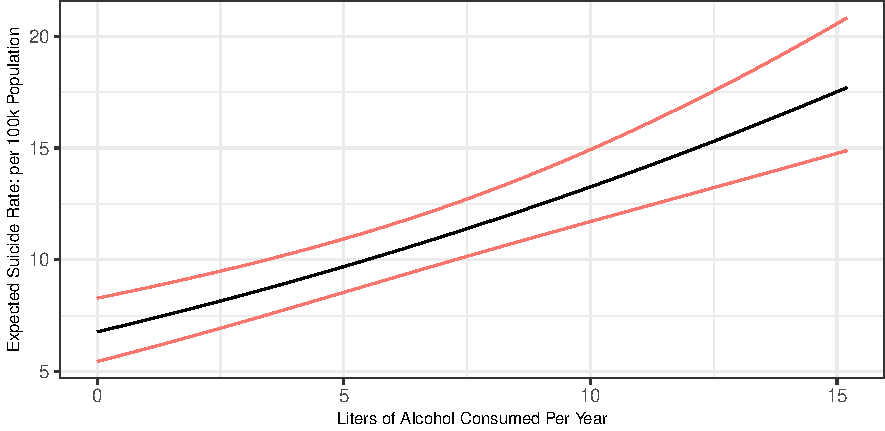
\includegraphics{Project_Report_files/figure-latex/a_alc_plot-1} \end{center}

\subsubsection{Quantifying Impact: The Presence of A National Suicide
Strategy}\label{quantifying-impact-the-presence-of-a-national-suicide-strategy}

Insights

Our model indicates that countries that have put a national suicide
prevention strategy in place, tend to have higher incidence of suicide
rates overall

Based on our estimates, countries that have implemented a suicide
prevention strategy have a 26\% higher incidence of suicide nationally

However, to put this in context, it appears that the institution of a
suicide prevention strategy by countries struggling with suicide
prevention overall, including Guyana, Lithuania, Suriname, Belarus and
South Korea are driving this estimate

\begin{center}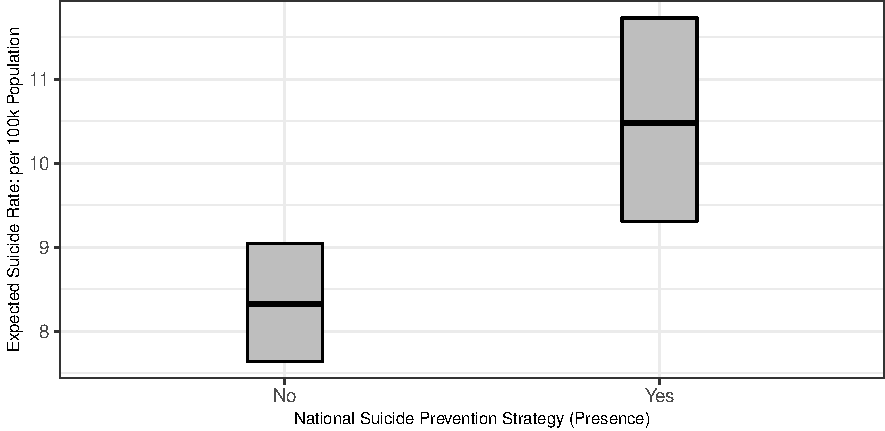
\includegraphics{Project_Report_files/figure-latex/sstrat_plot-1} \end{center}

\section{Research Limitations}\label{research-limitations}

\section{Appendix \& References}\label{appendix-references}

\emph{This section only includes needed documents to support the
presentation in the report. Feel free to divide it into several
subsections if necessary. Do NOT dump all computer outputs unor-ganized
here}

\subsection{Model Final Specification}\label{model-final-specification}

\[
\begin{aligned}
& Y_i = \beta_0 + \beta_1 x_{1i} + \beta_2 x_{2i} + \beta_3 x_{3i} + \beta_4 x_{4i}  + \epsilon_i,\ \text{where we assumed, } \epsilon_i \sim \mathbb{N}(0,\sigma_{Y}^2) \\
&\\
&\text{for } i = 1,...,n \ \text{country level measures, where} \\
& \\
& Y_i \ \ : \text{The estimated national suicide rate (per 100k population) for the} i^{\text{th}} \text{ country.(Box-cox transformed $\lambda = 0.4$)} \\
& x_{1i}\ : \text{The estimated national labor participation rate (percentage) for the } i^{\text{th}} \text{ country.}\\
& x_{2i}\ : \text{The log-transformed estimated per-person gross domestic product (GDP) (income) for the } i^{\text{th}} \text{ country.}\\
& x_{3i}\ : \text{An estimate of the national per-person average of liters of alcohol consumed annually for the } i^{\text{th}} \text{ country.}\\
& x_{4i}\ : \text{A binary indicator of the 'presence of a national suicide prevention strategy' in 2019 for the } i^{\text{th}} \text{ country.}\\
& \\
& \text{This yields fitted regression model: } \\
& \\
& \hat{Y_i} = \hat{\beta_0} + \hat{\beta_1} x_{1i} + \hat{\beta_2} x_{2i} + \hat{\beta_3} x_{3i} + \hat{\beta_4} x_{4i} \\
& \\
& \text{where, } \\
& \\
& \hat{\beta_0},\ \hat{\beta_1},\ \hat{\beta_2},\ \hat{\beta_3}, \ \text{and } \hat{\beta_4} \text{ were estimated by the method of iterative re-weighted least squares.} \\
\end{aligned}
\]

\subsection{Model Summary Statistics}\label{model-summary-statistics}

\begin{table}[H] \centering 
  \caption {Regression Model Summary} 
  \label{tab:title} 
\begin{tabular}{@{\extracolsep{5pt}}lc} 
\\[-1.8ex]\hline 
\hline \\[-1.8ex] 
 & \multicolumn{1}{c}{\textit{Dependent variable:}} \\ 
\cline{2-2} 
\\[-1.8ex] & Suicide Rate (Box-Cox Transformed $\lambda = 0.4$) \\ 
\hline \\[-1.8ex] 
 Income (pp GDP) - Log Transformed & $-$0.404$^{***}$ \\ 
  & (0.080) \\ 
  & \\ 
Liters of Alcohol Consumed & 0.166$^{***}$ \\ 
  & (0.026) \\ 
  & \\ 
Suicide Prevention Strategy (Binary) & 0.562$^{***}$ \\ 
  & (0.185) \\ 
  & \\ 
Labor Participation Rate & 1.031$^{**}$ \\ 
  & (0.472) \\ 
  & \\ 
 Constant & 5.420$^{***}$ \\ 
  & (0.828) \\ 
  & \\ 
\hline \\[-1.8ex] 
Observations & 162 \\ 
R$^{2}$ & 0.412 \\ 
Adjusted R$^{2}$ & 0.397 \\ 
Residual Std. Error & 1.272 (df = 157) \\ 
F Statistic & 27.475$^{***}$ (df = 4; 157) \\ 
\hline 
\hline \\[-1.8ex] 
\textit{Note:}  & \multicolumn{1}{r}{$^{*}$p$<$0.1; $^{**}$p$<$0.05; $^{***}$p$<$0.01} \\ 
\end{tabular} 
\end{table}

\newpage

\section*{References}\label{references}
\addcontentsline{toc}{section}{References}

\hypertarget{refs}{}
\hypertarget{ref-whodat2019}{}
``Suicide Rate Estimates, Age-Standardized Estimates by Country.'' 2019.
\url{http://apps.who.int/gho/data/node.main.MHSUICIDEASDR?lang=en}.

\hypertarget{ref-stats2019}{}
``Suicide: Key Facts.'' 2019.
\url{https://www.who.int/news-room/fact-sheets/detail/suicide}.

\hypertarget{ref-who2019}{}
``Suicide: One Person Dies Every 40 Seconds.'' 2019.
\url{https://www.who.int/news-room/detail/09-09-2019-suicide-one-person-dies-every-40-seconds}.

\end{document}
